\documentclass[11pt, twoside, pdftex]{article}

% This includes all the settings that we should use for the document
\newcommand{\PDFTitle}{Using TimeQuest Timing Analyzer}
\newcommand{\commonPath}{../../../Common}
\newcommand{\datePublished}{Mar 2022}

\newcommand{\versnum}{21.1} %version number quartus/AMP
\newcommand{\quartusname}{Quartus\textsuperscript{\textregistered} Prime}	
\newcommand{\textBar}{For \quartusname{} \versnum{}}
\newcommand{\thisyear}{2022 } %for copyright
\newcommand{\company}{FPGAcademy.org}
\newcommand{\longteamname}{FPGAcademy.org}
\newcommand{\teamname}{FPGAcademy}
\newcommand{\website}{FPGAcademy.org}

\newcommand{\productAcronym}{AMP}
\newcommand{\productNameShort}{Monitor Program}

\newcommand{\productNameMedTM}{Monitor Program}
\newcommand{\productNameMed}{Monitor Program}

%\newcommand{\headerLogoFilePath}[1]{#1/FPGAcademy.png}



\setlength\topmargin{-0.25in}
\setlength\headheight{0in}
\setlength\headsep{0.35in}
\setlength\textheight{8.5in}
\setlength\textwidth{7in}
\setlength\oddsidemargin{-0.25in}
\setlength\evensidemargin{-0.25in}
\setlength\parindent{0.25in}
\setlength\parskip{0in} 

\pdfpagewidth 8.5in
\pdfpageheight 11in

% listings is a package that supports encapsulating source code in LaTeX conveniently

\usepackage{listings}
% add support for graphics
\usepackage{graphicx}
\usepackage[usenames, dvipsnames]{color}

\def\expandparam\lstinputlisting[#1]#2{\edef\tmp{\noexpand\lstinputlisting[#1]{#2}}\tmp}

\widowpenalty 10000
\clubpenalty 10000

%%%%%%%%%%%%%%%%%%%% Source Code Formatting %%%%%%%%%%%%%%%%%%%%
\definecolor{globalCommentColour}{rgb}{0.588,0.588,0.588}

%%%%%%%%%%%%%%%%%%%%%%%%%%%%%%%%%%%%%%%%%%%%%%%%%%%%
% Defining a NiosII ASM highlighter for lstlisting
\lstdefinelanguage[NiosII]{Assembler} {
 	morekeywords={add, addi, and, andhi, andi, beq, bge, bgeu, bgt, bgtu, ble,  bleu, blt, bltu, bne, br, break,% 
 	bret, call, callr, cmpeq, cmpeqi, cmpge, cmpgei, cmpgeu, cmpgeui, cmpgt, cmpgti, cmpgtu, cmpgtui, cmple,%
 	cmplei, cmpleu, cmpleui, cmplt, cmplti, cmpltu, cmpltui, cmpne, cmpnei, custom, div, divu, eret, flushd,%
 	flushda, flushi, flushp, initd, initda, initi, jmp, jmpi, ldb, ldbio, ldbu, ldbuio, ldh, ldhio, ldhu, ldhuio,%
 	ldw, ldwio, mov, movhi, movi, movia, movui, mul, muli, mulxss, mulxsu, mulxuu, nextpc, nop, nor, or, orhi, ori,%
 	rdctl, rdprs, ret, rol, roli, ror, sll, slli, sra, srai, srl, srli, stb, stbio, sth, sthio, stw, stwio,%
 	sub, subi, sync, trap, wrctl, wrtcl, wrprs, xor, xori, xorhi, xori},% 	
 	morekeywords=[2]{.abort, .ABORT, .align, .app-file, .ascii, .asciz, .balign, .byte, .comm, .data, .def,%
 	.desc, .dim, .double, .eject, .else, .end, .endef, .endif, .equ, .equiv, .err, .extern, .file, .fill, .float,%
 	.global, .globl, .hword, .ident, .if, .include, .int, .irp, .irpc, .lcomm, .lflags, .line, .linkonce, .ln,%
 	.list, .long, .macro, .mri, .nolist, .octa, .org, .p2align, .psize, .quad, .rept, .sbttl, .scl, .section,%
 	.set, .short, .single, .size, .sleb128, .skip, .space, .stadb, .stabn, .stabs, .string, .symver, .tag,%
 	.text, .title, .type, .val, .uleb128, .word},% 	
 	morekeywords=[3]{et, bt, gp, sp, fp, ea, sstatus, ra, pc, status, estatus, bstatus, ienable, ipending, cpuid,%
 	exception, pteaddr, tlbacc, tlbmisc, eccinj, badaddr, config, mpubase, mpuacc},% 	
 	sensitive=t,%
 	alsoletter=.,%
	morestring=[b]",%
 	morecomment=[s]{/*}{*/},%
 	morecomment=[l]\#,%
   }[keywords,comments,strings]
   
   %% NOTE: morekeywords=[2] are GNU directives.
   
   \definecolor{niosInstructionColour}{rgb}{0.000,0.608,0.000}
   \definecolor{niosDirectiveColour}{rgb}{0.000,0.000,0.902}
   \definecolor{niosSpecialRegColour}{rgb}{0.000,0.000,0.000}
   \definecolor{niosStringColour}{rgb}{0.808,0.482,0.000}
   
   %% NOTE: To make bold use: =\bfseries\color{<colour>}
   \lstdefinestyle{defaultNiosStyle} {
   language=[NiosII]{Assembler},
   stringstyle=\color{niosStringColour},
   keywordstyle=\color{niosInstructionColour},
   keywordstyle=[2]\color{niosDirectiveColour},
   keywordstyle=[3]\itshape\color{niosSpecialRegColour}
   }
%%%%%%%%%%%%%%%%%%%%%%%%%%%%%%%%%%%%%%%%%%%%%%%%%%%%

%%%%%%%%%%%%%%%%%%%%%%%%%%%%%%%%%%%%%%%%%%%%%%%%%%%%
% Defining a ArmA9 ASM highlighter for lstlisting
\lstdefinelanguage[ArmA9]{Assembler} {
 	morekeywords={ADC, ADD, ADDS, AND, ANDS, B, BAL, BEQ, BGE, BGT, BL, BLT, BIC, BKPT, BLX, BNE, BX, CDP, CLZ, CMN, CMP, EOR,%
 	EORS, LDC, LDM, LDR, LDRB, LDRBT, LDRH, LDRSB, LDRSH, LDRT, LSL, MCR, MLA, MOV, MOVW, MOVT, MRC, MRS, MSR, MUL, MVN, ORR, PLD,%
 	ROR, RSB, RSC, SBC, SMLAL, SMULL, STC, STM, STR, STRB, STRBT, STRH, STRT, SUB, SUBS, SWI, SWP, SWPB, TEQ, UMLAL,
 	PUSH, POP, MOVS, RORS, LSR},%
 	morekeywords=[2]{.abort, .ABORT, .align, .app-file, .ascii, .asciz, .balign, .byte, .comm, .data, .def,%
 	.desc, .dim, .double, .eject, .else, .end, .endef, .endif, .equ, .equiv, .err, .extern, .file, .fill, .float,%
 	.global, .globl, .hword, .ident, .if, .include, .int, .irp, .irpc, .lcomm, .lflags, .line, .linkonce, .ln,%
 	.list, .long, .macro, .mri, .nolist, .octa, .org, .p2align, .psize, .quad, .rept, .sbttl, .scl, .section,%
 	.set, .short, .single, .size, .sleb128, .skip, .space, .stadb, .stabn, .stabs, .string, .symver, .tag,%
 	.text, .title, .type, .val, .vectors, .uleb128, .word},%
 	morekeywords=[3]{SP, PC, MIDR, CTR, TCMTR, TLBTR, MPIDR, ID_PFR0, ID_PFR1, ID_DFR0, ID_MMFR0, ID_MMFR1, ID_MMFR2,%
 	ID_MMFR3, ID_ISAR0, ID_ISAR1, ID_ISAR2, ID_ISAR3, ID_ISAR4, CCSIDR, CLIDR, AIDR, CSSELR, TTBR0, TTRB1, TTBR2, DACR,%
 	DFSR, IFSR, ADFSR, AIFSR, DFAAR, IFAR, ICIALLUIS, BPIALLIS, PAR, ICIALLU, ICIMVAU, BPIALL, DCIMVAC, DCISW, V2PCWPR,%
 	DCCVAC, DCCSW, DDIMVAC, DCISW, TLBALLIS, TLBIMVAIS, TLBIASIDIS, TLBIMVAAIS, TLBIALL, TLBIMVA, TLBIASID, TLBIMVAA,%
 	PMCR, PMCNTENSET, PMCNTENCLR, PMOVSR, PMSWINC, PMSELR, PMXEVTYPER, PMXEVCNTR, PMUSERENR, PMINTENSET, PMINTENCLR,%
 	PRRR, NRRR, PLEIDR, PLEASR, PLEFSR, PLEUAR, PLEPCR, VBAR, MVBAR, ISR, FCSEIDR, CONTEXTIDR, TPIDRURW, TPIDRURO, TPIDRPRW},%
 	sensitive=f,%
 	alsoletter=.,%
	morestring=[b]",%
 	morecomment=[s]{/*}{*/},%
 	morecomment=[l]{//},%
   }[keywords,comments,strings]
   
   %% NOTE: morekeywords=[2] are GNU directives.
   
   \definecolor{armInstructionColour}{rgb}{0.000,0.608,0.000}
   \definecolor{armDirectiveColour}{rgb}{0.000,0.000,0.902}
   \definecolor{armSpecialRegColour}{rgb}{0.000,0.000,0.000}
   \definecolor{armStringColour}{rgb}{0.808,0.482,0.000}
   
   \lstdefinestyle{defaultArmStyle} {
   language=[ArmA9]{Assembler},
   stringstyle=\color{armStringColour},
   keywordstyle=\color{armInstructionColour},
   keywordstyle=[2]\color{armDirectiveColour},
   keywordstyle=[3]\itshape\color{armSpecialRegColour}
   }
%%%%%%%%%%%%%%%%%%%%%%%%%%%%%%%%%%%%%%%%%%%%%%%%%%%%

%%%%%%%%%%%%%%%%%%%%%%%%%%%%%%%%%%%%%%%%%%%%%%%%%%%%
% Defining style for the verilog.

\definecolor{verilogCommentColour}{rgb}{0.000,0.502,0.000}

\lstdefinestyle{defaultVerilogStyle} {
language={Verilog},
keywordstyle=\color{blue},
commentstyle=\color{verilogCommentColour}
}
%%%%%%%%%%%%%%%%%%%%%%%%%%%%%%%%%%%%%%%%%%%%%%%%%%%%

%%%%%%%%%%%%%%%%%%%%%%%%%%%%%%%%%%%%%%%%%%%%%%%%%%%%
% Defining style for the vhdl.
\lstdefinestyle{defaultVHDLStyle} {
language={VHDL},
keywordstyle=\color{blue},
commentstyle=\color{verilogCommentColour}
}
%%%%%%%%%%%%%%%%%%%%%%%%%%%%%%%%%%%%%%%%%%%%%%%%%%%%

%%%%%%%%%%%%%%%%%%%%%%%%%%%%%%%%%%%%%%%%%%%%%%%%%%%%
% Java
\definecolor{javaStringColour}{rgb}{0.808,0.482,0}
%%%%%%%%%%%%%%%%%%%%%%%%%%%%%%%%%%%%%%%%%%%%%%%%%%%%

%%%%%%%%%%%%%%%%%%%%%%%%%%%%%%%%%%%%%%%%%%%%%%%%%%%%
% Defining language styles
% C
\definecolor{CStringColour}{rgb}{0.808,0.482,0}
%%%%%%%%%%%%%%%%%%%%%%%%%%%%%%%%%%%%%%%%%%%%%%%%%%%%

%%%%%%%%%%%%%%%%%%%%%%%%%%%%%%%%%%%%%%%%%%%%%%%%%%%%
% Defining extended LaTeX language.
\lstdefinelanguage[LocalLaTeX]{TeX}[LaTeX]{TeX}%
 	{moretexcs={bf, it, sf, lstset},%
   	}%

\lstdefinestyle{defaultLocalLatexStyle} {
language=[LocalLatex]{TeX},
keywordstyle=\color{blue}\bfseries,
keywordstyle=[2]\color{blue},
keywordstyle=[3]\color{blue}\bfseries
}
%%%%%%%%%%%%%%%%%%%%%%%%%%%%%%%%%%%%%%%%%%%%%%%%%%%%

\lstset{
%language = C,
%language = Verilog,
%basicstyle=\color{black}\rmfamily\ttfamily,
basicstyle=\small\color{black}\ttfamily,
commentstyle=\small\color{globalCommentColour}\itshape\ttfamily,
keywordstyle=\small\color{blue}\bfseries\ttfamily,
showstringspaces=false,
frame=none, %lines % boxed listings
breaklines=true,
breakatwhitespace=true,
tabsize=4
}
%%%%%%%%%%%%%%%%%%%%%%%%%%%%%%%%%%%%%%%%%%%%%%%%%%%%%%%%%%%%%%%%


%\usepackage[centering]{geometry}.
%%%%%%%%%%%%%%%%%%%%%%%%%%%%%%%%%%%%%%%%%%%%%%%%%%%
% Document Settings
\usepackage[labelsep=period]{caption}
% we can choose a better font later
%\usepackage{palatino}
\usepackage{fourier}
%\fontencoding{T1}
% include common used symbols
\usepackage{textcomp}
% add support for graphics
\usepackage{graphicx}
\usepackage[usenames, dvipsnames]{color}
% enable to draw thick or thin table hlines
\setlength{\doublerulesep}{\arrayrulewidth}
\usepackage{longtable}
\setlongtables
%\usepackage{array}
% It may be better to use PDFLaTeX as it can generate bookmarks for the
% document

% Add some useful packages
\usepackage{ae,aecompl}
\usepackage{epsfig,float,times}

% reset the font for section
\usepackage{sectsty}
%\allsectionsfont{\fontfamily{ptm}\selectfont}
\allsectionsfont{\usefont{OT1}{phv}{bc}{n}\selectfont}

% use compact space for sections
\usepackage[compact]{titlesec}
\titlespacing{\section}{0pt}{0.2in}{*0}
\titlespacing{\subsection}{0pt}{0.1in}{*0}
\titlespacing{\subsubsection}{0pt}{0.05in}{*0}

% fancyhdr header and footer customization
\usepackage{layout}
\usepackage{fancyhdr}
\pagestyle{fancy}
\fancyhead{}
\fancyhead[R]{\textit{\tiny{\textBar}}}
\fancyfoot{}
\fancyfoot[LO,
RE]{\textrm{\href{https://www.fpgacademy.org}{\small \longteamname}} \\ {\small \datePublished }}
\fancyfoot[RO, LE]{\small \thepage}
% two-side settings
%\fancyhead{} % clear all header fields
%\fancyfoot{} % clear all footer fields
%\fancyfoot[LE,RO]{\thepage}
\renewcommand{\headrulewidth}{2pt}
\renewcommand{\headrule}{{\color{blue} \hrule width\headwidth height\headrulewidth \vskip-\headrulewidth}}
\renewcommand{\footrulewidth}{0pt}

% Format the footer on page 1
\fancypagestyle{plain}{
\fancyhead{}
\fancyfoot{}
\fancyfoot[LO,
RE]{\textrm{\href{https://www.fpgacademy.org}{\small \longteamname}} \\ {\small \datePublished }}
\fancyfoot[RO, LE]{\small \thepage}
\renewcommand{\headrulewidth}{0pt}
}
% adjust some setting to try to make the figure stay in the same page with text
% Reference: 	http://www.cs.uu.nl/~piet/floats/node1.html
%   			http://mintaka.sdsu.edu/GF/bibliog/latex/floats.html
%   General parameters, for ALL pages:
\renewcommand{\topfraction}{0.9}	% max fraction of floats at top
\renewcommand{\bottomfraction}{0.8}	% max fraction of floats at bottom
%   Parameters for TEXT pages (not float pages):
\setcounter{topnumber}{3}
\setcounter{bottomnumber}{3}
\setcounter{totalnumber}{5}     % 2 may work better
\setcounter{dbltopnumber}{2}    % for 2-column pages
\renewcommand{\dbltopfraction}{0.9}	% fit big float above 2-col. text
\renewcommand{\textfraction}{0.07}	% allow minimal text w. figs
%   Parameters for FLOAT pages (not text pages):
\renewcommand{\floatpagefraction}{0.7}	% require fuller float pages
% N.B.: floatpagefraction MUST be less than topfraction !!
\renewcommand{\dblfloatpagefraction}{0.7}	% require fuller float pages
%%%%%%%%%%%%%%%%%%%%%%%%%%%%%%%%%%%%%%%%%%%%%%%%%%%
% remember to use [htp] or [htpb] for placement
%%%%%%%%%%%%%%%%%%%%%%%%%%%%%%%%%%%%%%%%%%%%%%%%%%%

% set no indent for paragraph
\setlength{\parindent}{0em}
\addtolength{\parskip}{11pt}
\newcommand{\compact}{[topsep=0pt]}
% use this package to reduce space
\usepackage{enumitem}
\usepackage{multirow}
\usepackage{rotating}
\usepackage{pifont}
\usepackage{dingbat}
\newcommand{\itemsecond}{$\circ$}
%
%%%%%%%%%%%%%%%%%%
\date{}
\author{}
%%%%%%%%%%%%%%%%%%
\newcommand{\de}{DE-series}
\newcommand{\up}{FPGAcademy}
\newcommand{\fabric}{Avalon Switch Fabric}
\newcommand{\TODO}[1]{\textcolor{red}{\textbf{TODO}: #1}}
\def\registered{{\ooalign{\hfil\raise .00ex\hbox{\scriptsize R}\hfil\crcr\mathhexbox20D}}}

% enable url and reference(bookmarks) in pdf
\usepackage{url}
\usepackage[pdftex, colorlinks]{hyperref}
\hypersetup{%
pdftitle={\PDFTitle},
linkcolor=blue,
hyperindex=true,
pdfauthor={\longteamname},
pdfkeywords={FPGAcademy, Academic Program, Example System},
bookmarksnumbered,
bookmarksopen=false,
filecolor=blue,
pdfstartview={FitH},
urlcolor=blue,
plainpages=false,
pdfpagelabels=true,
linkbordercolor={1 1 1} %no color for link border
}%
%%%%%%%%%%%%%%%%%%%%%%%%%%%%%%%%%%%%%%%%%%%%%%%%%%%
\setlength{\fboxsep}{0.7pt}
\setlength{\fboxrule}{0.5pt}

\newcommand{\red}[1]{{\color{red}\sf{#1}}}
\newcommand{\blue}[1]{{\color{blue}\sf{#1}}}



%%%%%%%%%%%%%%%%%%%%%%%%%
% Add title
\newcommand{\doctitle}{Using TimeQuest \\ Timing Analyzer}
\newcommand{\dochead}{Using TimeQuest Timing Analyzer}
% Usually no need to change these two lines
\title{\fontfamily{phv}\selectfont{\doctitle} }
\chead{ \small{\textsc{\bfseries \dochead} } }
% Customizations
%%%%%%%%%%%%%%%%%%%%%%%%%
% Allows multiple figures per page

\renewcommand\floatpagefraction{.9}
\renewcommand\topfraction{.9}
\renewcommand\bottomfraction{.9}
\renewcommand\textfraction{.1}   
\setcounter{totalnumber}{50}
\setcounter{topnumber}{50}
\setcounter{bottomnumber}{50}
\widowpenalty 10000
\clubpenalty 10000
\raggedbottom

%%%%%%%%%%%%%%%%%%
%%% DOCUMENT START
%\begin{document}
\begin{document}
\begin{table}
    \centering
    \begin{tabular}{p{5cm}p{4cm}}
        \hspace{-3cm}
        &
        \raisebox{1\height}{\parbox[h]{0.5\textwidth}{\Large\fontfamily{phv}\selectfont{\textsf{\doctitle}}}}
    \end{tabular}
    \label{tab:logo}
\end{table}

\colorbox[rgb]{0,0.384,0.816}{\parbox[h]{\textwidth}{\color{white}\textsf{\textit{\textBar}}}}

\thispagestyle{plain}
 
\section{Introduction}

This tutorial provides an introduction to TimeQuest Timing Analyzer. It demonstrates how to 
set up timing constraints and obtain timing information for a logic circuit.

The reader is expected to have a basic understanding of the VHDL hardware description 
language, and to be familiar with the Intel\textsuperscript{\textregistered} Quartus\textsuperscript{\textregistered} Prime CAD software.

{\bf Contents}:
\begin{itemize}
\item Introduction to timing analysis
\item Using TimeQuest
\item Setting Up Timing Constraints
\end{itemize}
\clearpage
\newpage

\section{Background}

Timing analysis is a process of analyzing delays in a logic circuit to determine the conditions 
under which the circuit operates reliably. One example of a timing analysis computation is
to find the maximum clock frequency for a circuit, illustrated in 
Figure~\ref{fig:fmax_computation_example}. 

\begin{figure}[H]
\begin{center}
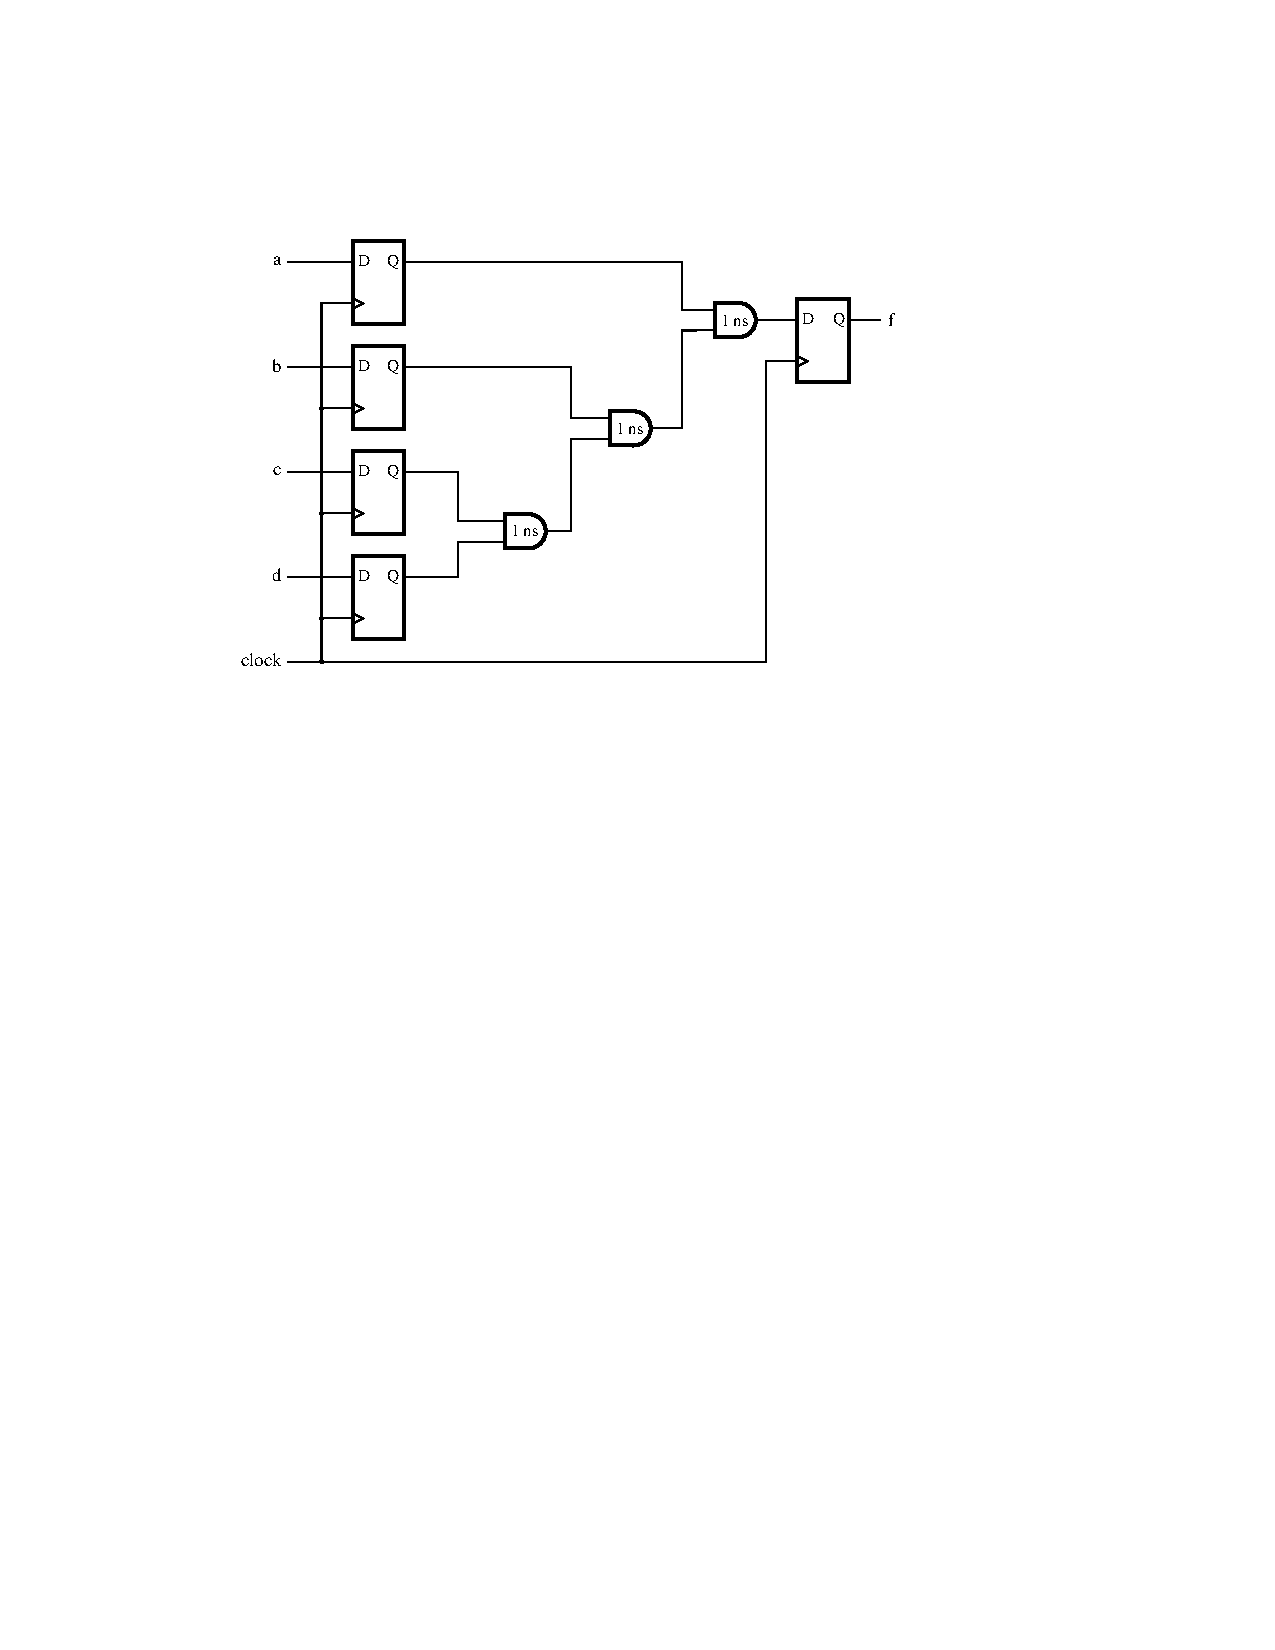
\includegraphics[scale=.75]{figures/sample_circuit_unbalanced.pdf}
\end{center}
\caption{A example for timing analysis.}
\label{fig:fmax_computation_example}
\end{figure}

\noindent
In this example, flip-flops on the left-hand side drive a combinational circuit that 
generates an output that is later stored in the flip-flop on the right-hand side. To 
operate correctly, the clock period has to be long enough to accommodate the delay on the 
longest path in the circuit. If we assume that the clock-to-Q and setup times for each 
flip-flop are 1 ns, and the delay through each gate is 1 ns, then the maximum clock frequency 
for this circuit is:
$$
f_{max} = \frac{1}{t_{cq}+3 \times t_{and}+t_{su}} = \frac{1}{5 {\rm ~ns}} = 200 {\rm ~MHz}
$$
Computing the longest delays in a circuit and comparing these delays to the clock period 
is a basic function of a timing analyzer. The timing analyzer can be used to guide 
computer-aided design (CAD) tools in the implementation of logic circuits. For example, the 
circuit in Figure~\ref{fig:fmax_computation_example} shows an implementation
of a 4-input function using 2-input AND gates. Without any timing requirements, the presented solution is acceptable. However, if a user
requires the circuit to operate at a clock frequency of 250 MHz, then 
the above solution is inadequate. By placing timing constraints on the
maximum clock frequency, it is possible to direct the CAD tools to seek an implementation
that meets those constraints. As a result,
the CAD tools may arrive at a solution shown in Figure~\ref{fig:fmax_computation_example_optimized}. The new circuit has
$f_{max} = 250$ MHz and thus meets the required timing constraints.

\begin{figure}[H]
\begin{center}
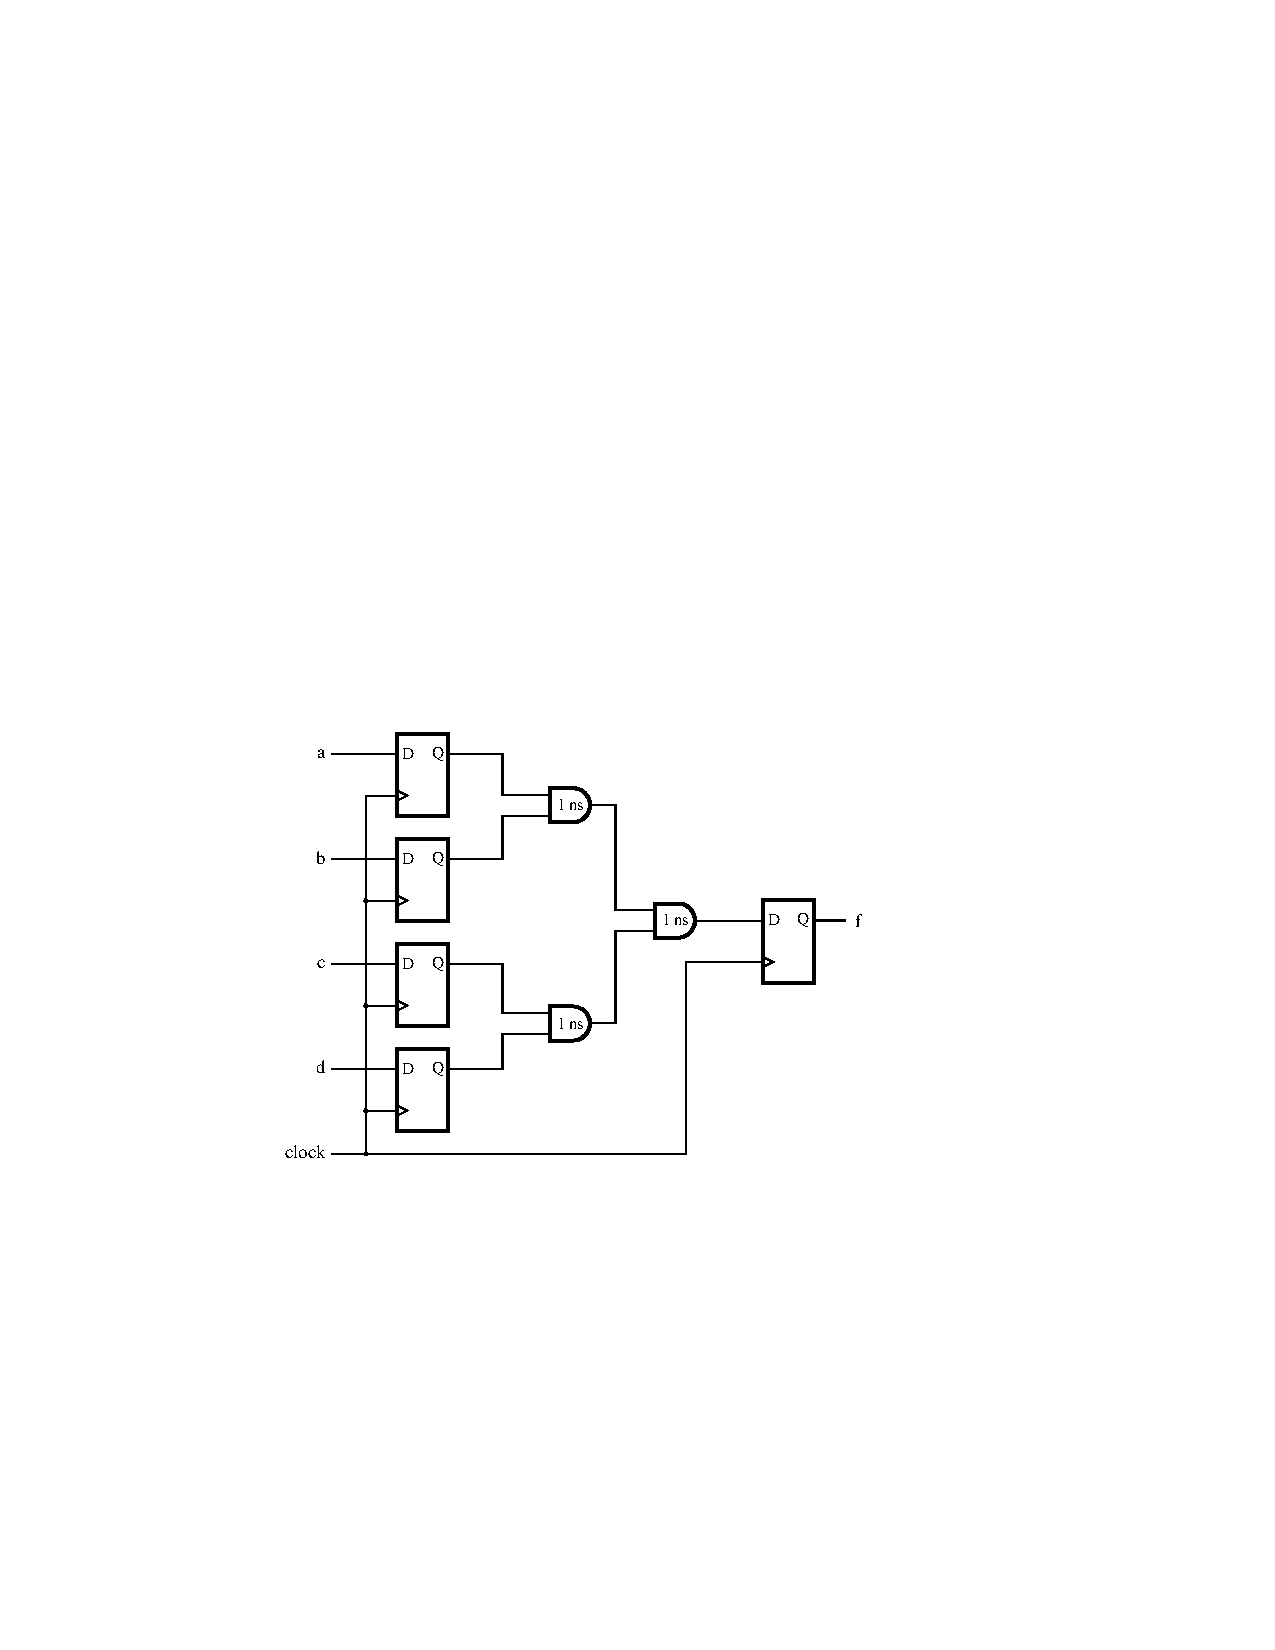
\includegraphics[scale=.75]{figures/sample_circuit_balanced.pdf}
\end{center}
\caption{Functionally equivalent circuit with a different logic structure.}
\label{fig:fmax_computation_example_optimized}
\end{figure}

In this tutorial, we demonstrate how to obtain timing information and how to set timing 
constraints using the TimeQuest timing analyzer.

The example circuit provided with this tutorial contains only one clock signal, which is
connected to all flip-flops. Performing timing analysis for circuits that have
multiple clock signals is discussed in section \ref{sec:mult}.

\section{Design Example}
As an example we will use an adder that adds three 8-bit numbers and produces a sum output. The inputs are $A$, $B$, and $C$, which are
stored in registers {\it reg\_A}, {\it reg\_B} and {\it reg\_C} at the positive edge of the {\it clock}. The three registers provide inputs
to the adder, whose result is stored in the {\it reg\_sum} register. The output of the {\it reg\_sum} register drives
the output port {\it sum}. The diagram of the circuit is shown in Figure~\ref{fig:design_example}.

\begin{figure}[H]
\begin{center}
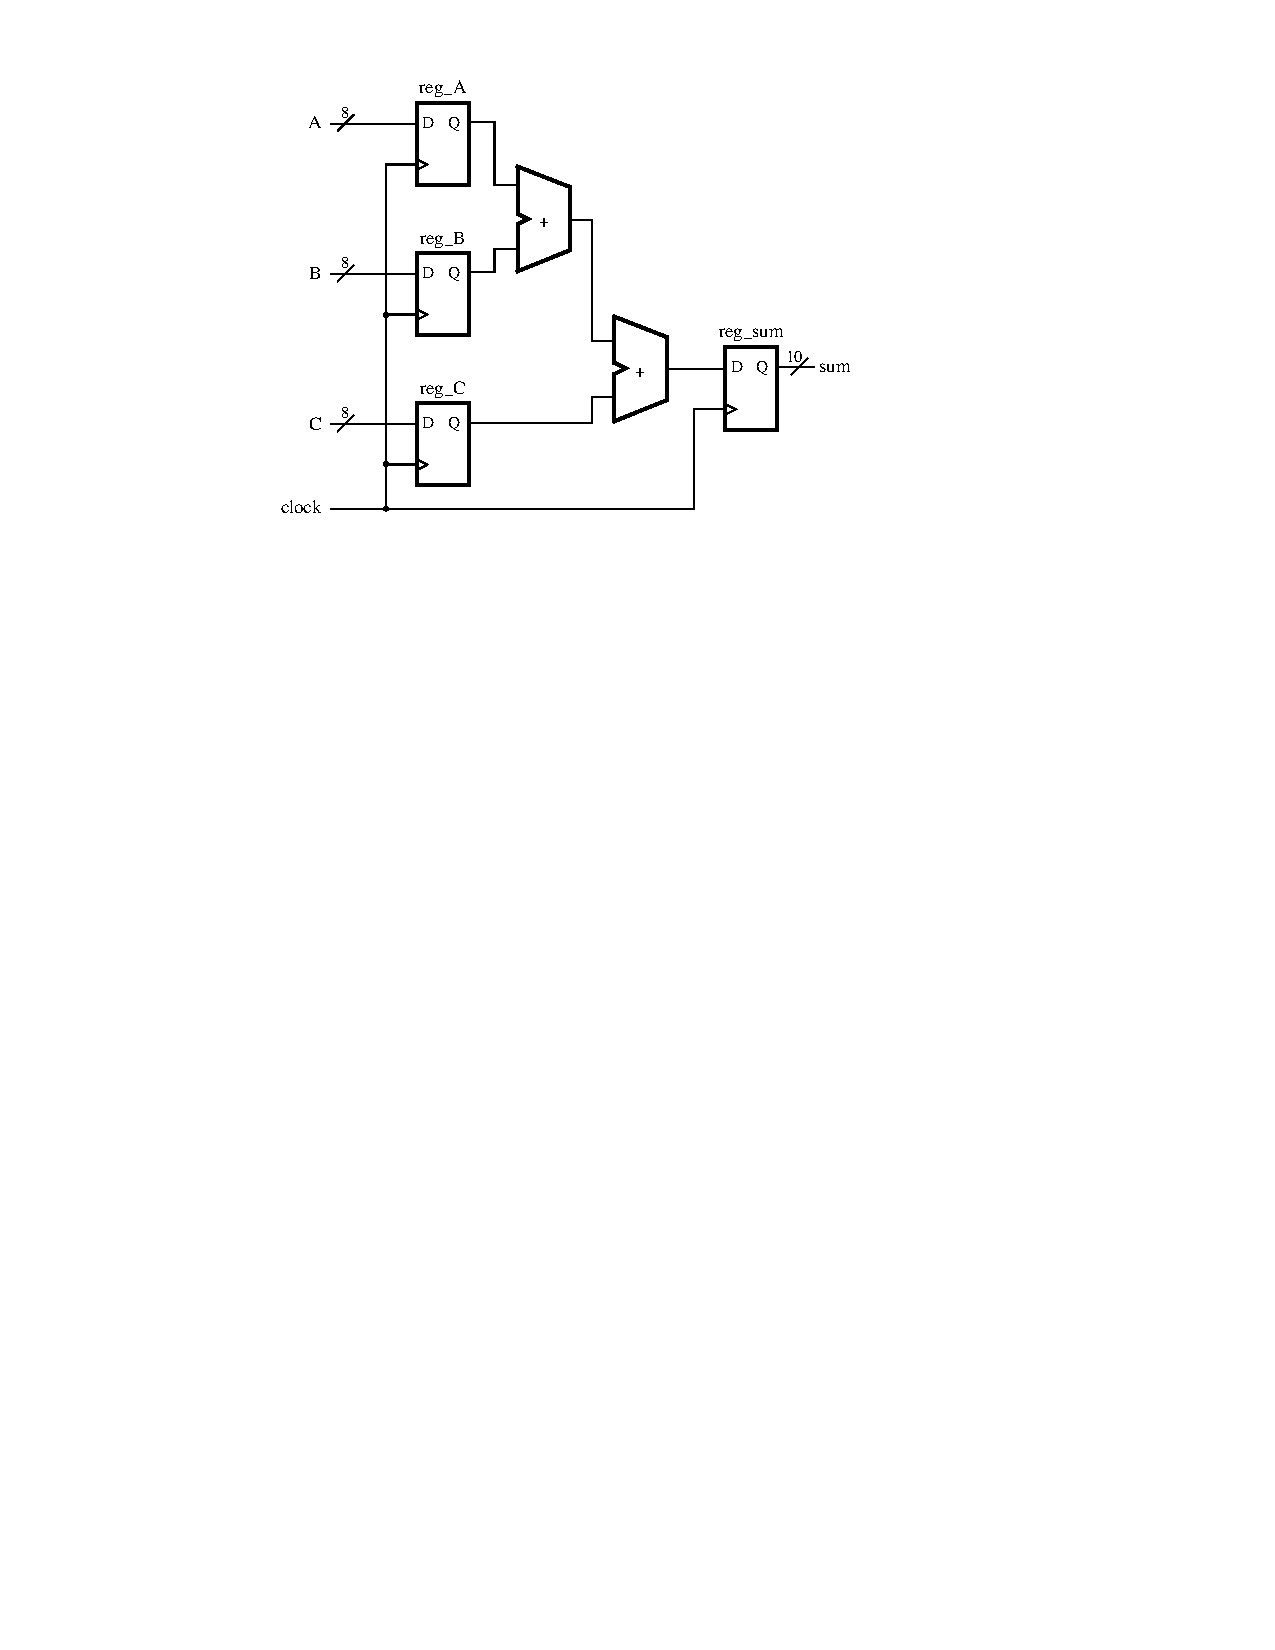
\includegraphics[scale=.75]{figures/design_example.pdf}
\end{center}
\caption{Diagram of the example circuit.}
\label{fig:design_example}
\end{figure}

The VHDL source code for the design is given in Figure~\ref{fig:design_VHDL_code}. Note that the ''synthesis keep''
comment is included in this code. This comment is interpreted as a directive that
instructs the Quartus Prime software to retain the specified
nodes in the final implementation of the circuit and keep their names as stated. This directive will allow us to refer to these nodes
in the tutorial. 

\begin{figure}[H]
\begin{lstlisting}[language=VHDL]
LIBRARY ieee;
USE ieee.std_logic_1164.all;
USE ieee.std_logic_unsigned.all;

ENTITY add_three_numbers IS
    PORT ( clock : IN STD_LOGIC;
        A, B, C  : IN STD_LOGIC_VECTOR(7 DOWNTO 0);
        sum      : OUT STD_LOGIC_VECTOR(9 DOWNTO 0));
END add_three_numbers;

ARCHITECTURE Behavior OF add_three_numbers IS
    -- Registers
    SIGNAL reg_A, reg_B, reg_C : STD_LOGIC_VECTOR(7 DOWNTO 0);
    SIGNAL reg_sum             : STD_LOGIC_VECTOR(9 DOWNTO 0);
    ATTRIBUTE keep             : boolean;
    ATTRIBUTE keep OF reg_A, reg_B, reg_C, reg_sum : SIGNAL IS true;
BEGIN
    PROCESS ( clock )
    BEGIN
        IF (clock'EVENT AND clock = '1') THEN
            reg_A <= A;
            reg_B <= B;
            reg_C <= C;
            reg_sum <= ("00" & reg_A) + ("00" & reg_B) + ("00" & reg_C);
        END IF;
    END PROCESS;

    sum <= reg_sum;
END Behavior;
\end{lstlisting}
\caption{VHDL code for the example circuit.}
\label{fig:design_VHDL_code}
\end{figure}

To begin the tutorial create a new Quartus Prime project for the design of our example circuit. 
Select as the target device the EP4CE115F29C7, which is the FPGA chip on the Intel DE2-115 
board. Type the VHDL code in Figure~\ref{fig:design_VHDL_code} into a file and add
this file to the project. 

You do not need to make any pin assignments for this example.  Compile the project to see the 
results of timing analysis. These results will be available in the compilation
report, once the design is compiled. 

\section{Using TimeQuest}

As illustrated in Figure~\ref{fig:SB1}, open the Timequest Timing Analyzer section 
of the Compilation Report, and click on the {\sf Clocks} item to select it. 
In the {\it Clocks} display panel that opens on the right-hand side of the Quartus Prime
window, notice that the {\it clock} signal from the example design 
has been given a clock period constraint of 1 ns (frequency of 1000 MHz). This is a
default constraint that the Quartus Prime CAD tool places on any clock signal in a design project
that does not have any user-provided timing constraints. 

\begin{figure}[H]
\begin{center}
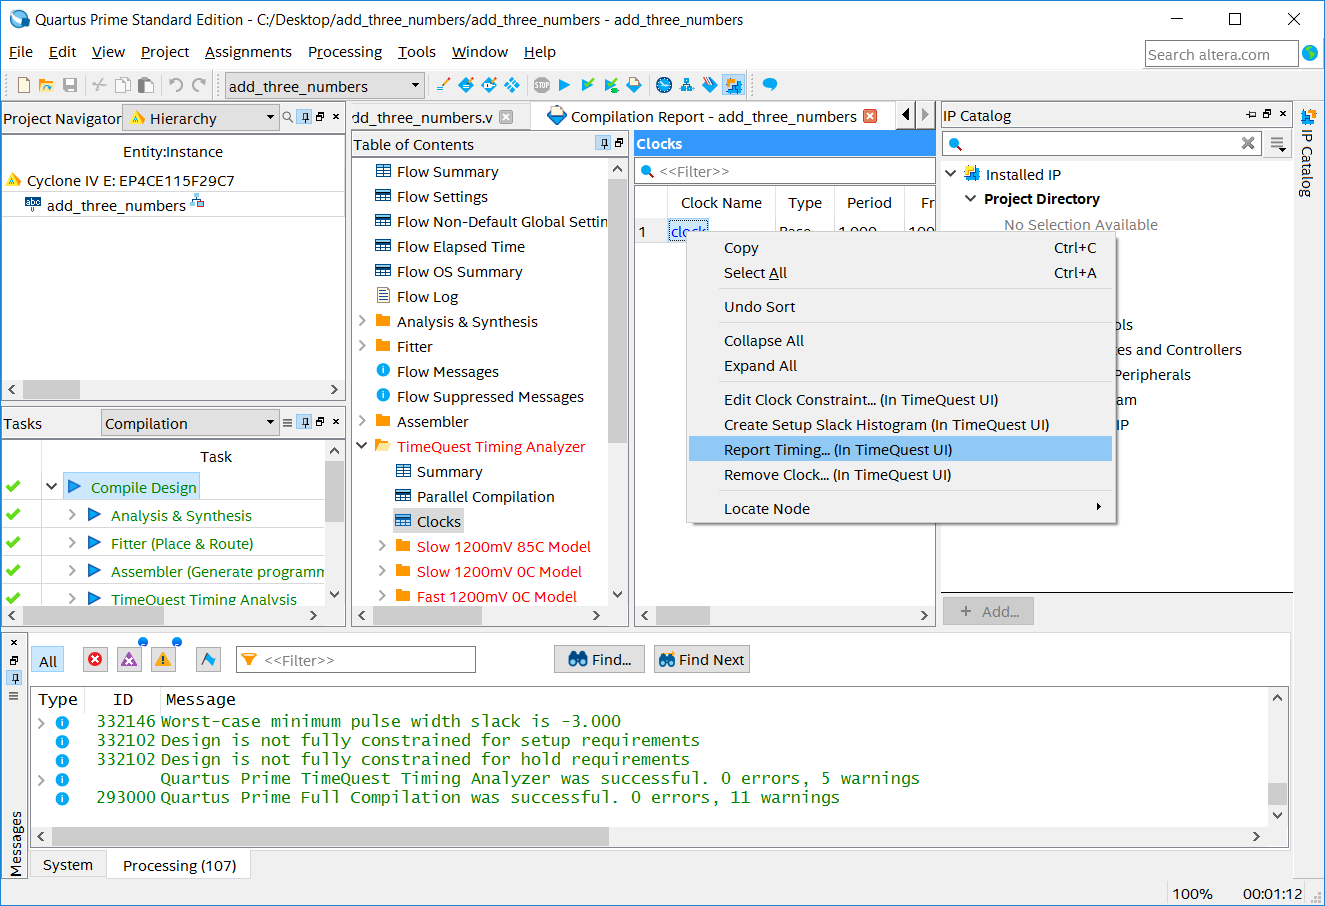
\includegraphics[scale=0.5]{figures/SB1.png}
\end{center}
\caption{The Timequest section of the compilation report.}
\label{fig:SB1}
\end{figure}

As indicated in Figure~\ref{fig:SB1}, right-click on the name of the {\it clock} signal 
and select the command {\sf Report Timing ... (In Timequest UI)}. This action opens
the {\it Report Timing} dialog shown in Figure~\ref{fig:SB2}. Click the drop-down arrow
in the {\sf From clock} item and select the {\it clock} signal. This selection is used to
instruct TimeQuest to analyze all paths in the example circuit that start and end at
flip-flops that are clocked by the {\it clock} signal. The various settings displayed in 
Figure~\ref{fig:SB2} are described in Section \ref{sec:TQGUI}.

Accept all of the other default selections in Figure~\ref{fig:SB2} and click on 
the {\sf Report Timing} button. This command opens the Timequest Graphical User Interface
(GUI), as depicted in Figure \ref{fig:SB3}.

\begin{figure}[H]
\begin{center}
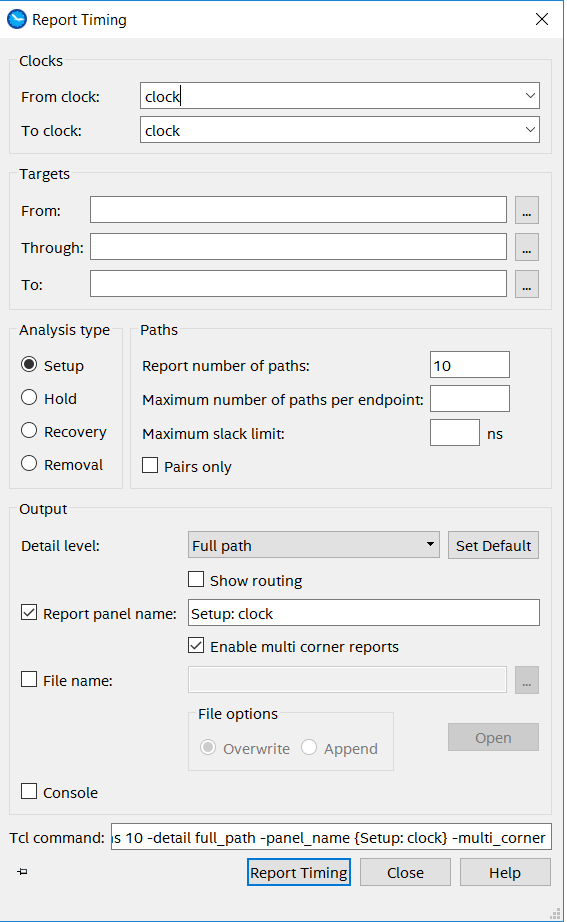
\includegraphics[scale=0.6]{figures/SB2.png}
\end{center}
\caption{The Report Timing dialog.}
\label{fig:SB2}
\end{figure}

\begin{figure}[H]
\begin{center}
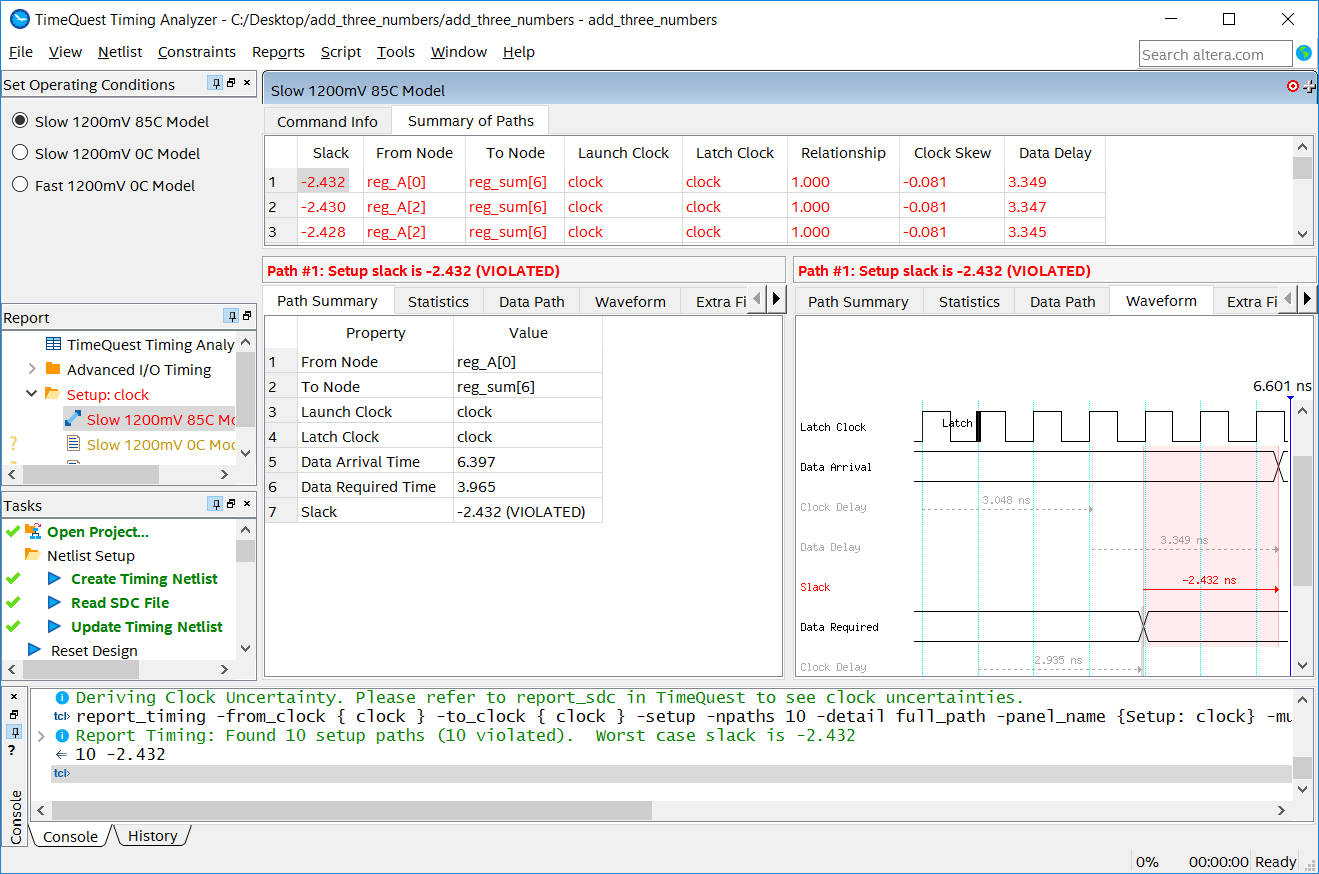
\includegraphics[scale=0.5]{figures/SB3.png}
\end{center}
\caption{The TimeQuest GUI.}
\label{fig:SB3}
\end{figure}

The TimeQuest GUI consists of several sections. They include the main menu at the top, the 
Report pane in the top-left corner, the Tasks pane on the left, the detailed results panes
in the middle, and the Console display at the bottom of the window. The main menu is used 
to interact with the TimeQuest tool and issue commands. The Report pane contains any 
reports generated when 
using the tool, and the Tasks pane contains a sequence of actions that can be performed to
obtain timing reports. The View pane hosts any windows that are opened, such as details
about the timing information.  The Console window at the bottom provides access to a command 
line for TimeQuest.

We will focus on the panes in the middle of the TimeQuest GUI, which show detailed
results of the timing analysis. The {\sf Slow 1200mV 85C Model} pane lists the analyzed paths in the 
circuit from source to destination flip-flops. The first column in this pane shows the
{\it Slack} of each path with respect to the (default) clock constraint of 1 ns.  For each
path in the circuit the slack value represents the difference between the clock period 
constraint and the path delay; a positive slack means that the delay is smaller than the 
constraint, and a negative slack represents a delay that is larger than the constraint. 
The slack values in the report are negative, and shown in red, because the timing results 
fail to meet the required constraint.  The maximum negative slack value shown is -2.432 ns, 
which means that the worst-case delay path is $1 - (-2.432) = 3.432$ ns long. This corresponds 
to a maximum usable clock frequency, F$_{max}$, of about 291.38 MHz.

The waveforms shown for path \#1 in Figure \ref{fig:SB3} illustrate the detailed timing
situation. The waveforms show that the clock signal takes 3.048 ns to propagate from its
input pin to the source flip-flop, and then this flip-flop produces data that takes 3.349 ns to reach the
destination flip-flop. Also, the clock signal takes 2.935 ns to reach the destination
flip-flop. The clock delays at the source and destination flip-flops
represent a clock skew $t_{skew} = 2.935 - 3.048 = -0.113$. A value of $0.032$
to account for {\it Clock Pessimism} is added to the clock skew, 
making the final clock skew value to be -0.081 ns.
The difference in the required arrival time of the data on this path and the
actual arrival time is shown by the negative slack value of 
$1 - 3.349 + t_{skew} = -2.430$ ns. TimeQuest adds a value of $-0.002$ ns to account for 
{\it Clock Uncertainty}, leading to the final slack value of -2.432 ns.

\subsection{Setting Up Timing Constraints for a Design}
In the TimeQuest GUI, select {\sf Constraints $>$ Create Clock}, which leads to the
Create Clock window shown in Figure~\ref{fig:setconstraint1}. Set the Clock name to
{\it clock} and the Period to {\it 4.000} ns. It is necessary to tell TimeQuest which signal in
our design this clock constraint applies to. To do this, click the {\sf ...} button to the right of 
the {\sf Targets} field, leading to the Name Finder window shown in Figure~\ref{fig:setconstraint2}.
Click {\sf List} to show all of the ports in the design. In the list of ports, highlight {\it clock}, which is the
clock signal in our circuit, press {\sf $>$}, then click {\sf OK}. Finally, click the {\sf Run}
button in the Create Clock window to apply the constraint.

In order to use this clock constraint for all future compilations and timing 
analysis of this project, we must save the constraint to a file of the type
{\it sdc} which stands for {\sf Synopsys* Design Constraint}. This file uses an industry-standard
format for specifying timing constraints. Select {\sf Constraints $>$ Write SDC File...} to write
all of the currently set constraints (in our case just the one clock constraint) to an SDC file.
This leads to the dialog shown in Figure~\ref{fig:setconstraint4}. Specify the file name {\it add\_three\_numbers.sdc}
and press {\sf OK}. Note that Quartus will by default try to locate and use the sdc file whose file name
matches the project name (except for the .sdc extension).

You will notice that our clock timing report {\it Setup clock} is now out of date, as indicated by the yellow
font and highlighting. Right-click the report and select {\sf Regenerate}, as shown in 
Figure~\ref{fig:setconstraint5}, to re-run the timing analysis using the new 4 ns clock period constraint. 
This analysis results in a positive slack of 0.568 ns. The corresponding waveforms are depicted in 
Figure~\ref{fig:SB8}. 

\begin{figure}[H]
\begin{center}
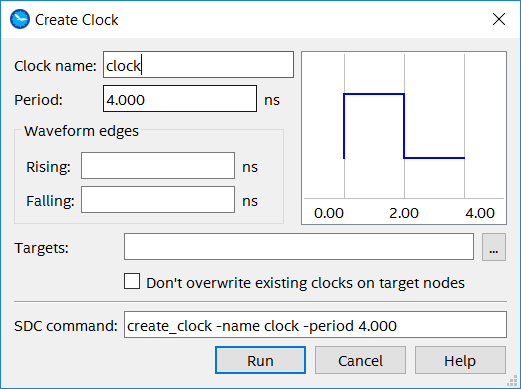
\includegraphics[scale=0.55]{figures/setconstraint1.png}
\end{center}
\caption{The Create Clock window.}
\label{fig:setconstraint1}
\end{figure}

\begin{figure}[H]
\begin{center}
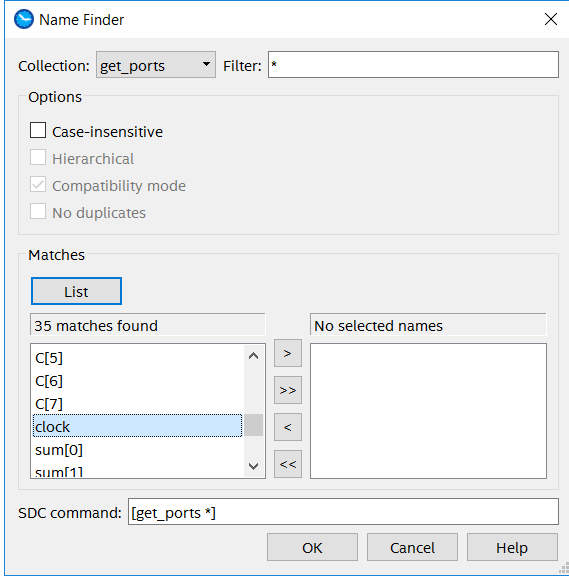
\includegraphics[scale=0.55]{figures/setconstraint2.png}
\end{center}
\caption{The Name Finder window.}
\label{fig:setconstraint2}
\end{figure}

\begin{figure}[H]
\begin{center}
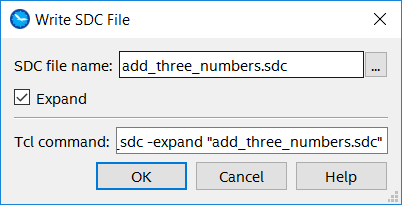
\includegraphics[scale=0.55]{figures/setconstraint4.png}
\end{center}
\caption{The Write SDC File dialog.}
\label{fig:setconstraint4}
\end{figure}

\begin{figure}[H]
\begin{center}
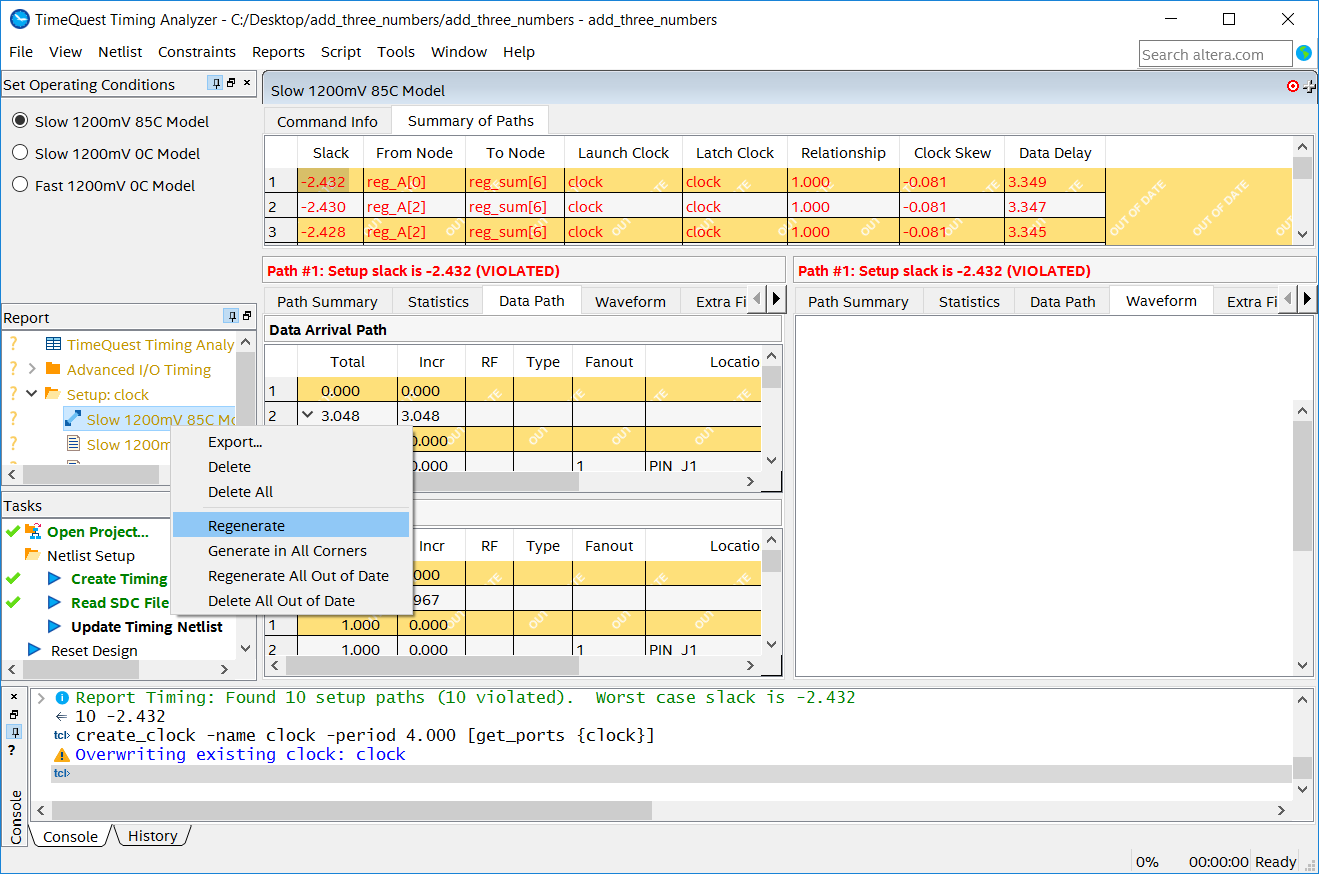
\includegraphics[scale=0.5]{figures/setconstraint5.png}
\end{center}
\caption{Regenerating the Timing Report.}
\label{fig:setconstraint5}
\end{figure}

\begin{figure}[H]
\begin{center}
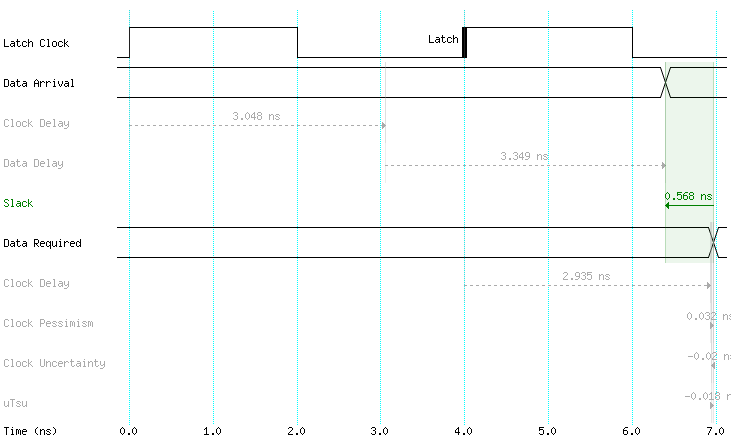
\includegraphics[scale=0.55]{figures/SB8.png}
\end{center}
\caption{Timing analysis results using the 4 ns clock period constraint.}
\label{fig:SB8}
\end{figure}

Close the TimeQuest GUI. A dialog will appear, asking if you want to save the SDC file.
Select {\sf No}, since we have already saved the SDC file.

Since we have not recompiled the example design after adding the 4 ns clock period
constraint, the timing analysis is based of the circuit that was produced by Quartus Prime
when using the (default) 1 ns clock period constraint. To see the effect of the new timing
constraint on the compilation results, recompile the project. Then, follow the steps described
previously to perform a new timing analysis using TimeQuest. The 4 ns timing constraint
will cause the Quartus Prime optimization algorithms to make different decisions from those
made when the (default) 1 ns constraint was used. In particular, the optimization
algorithms will likely take less time to execute, because once the generated circuit has
sufficient positive slack to meet the constraint, the algorithms can terminate. 
Figure~\ref{fig:SB9} shows the results of timing analysis, with a positive slack of 0.718 ns. 
If the constraint is not in effect after recompilation, you need to add the saved SDC file to the project.
On the left side under Task section, expand Timing Analysis and click on Edit Setting to add the saved SDC file to the project and then recompile and follow the previous steps.

\begin{figure}[H]
\begin{center}
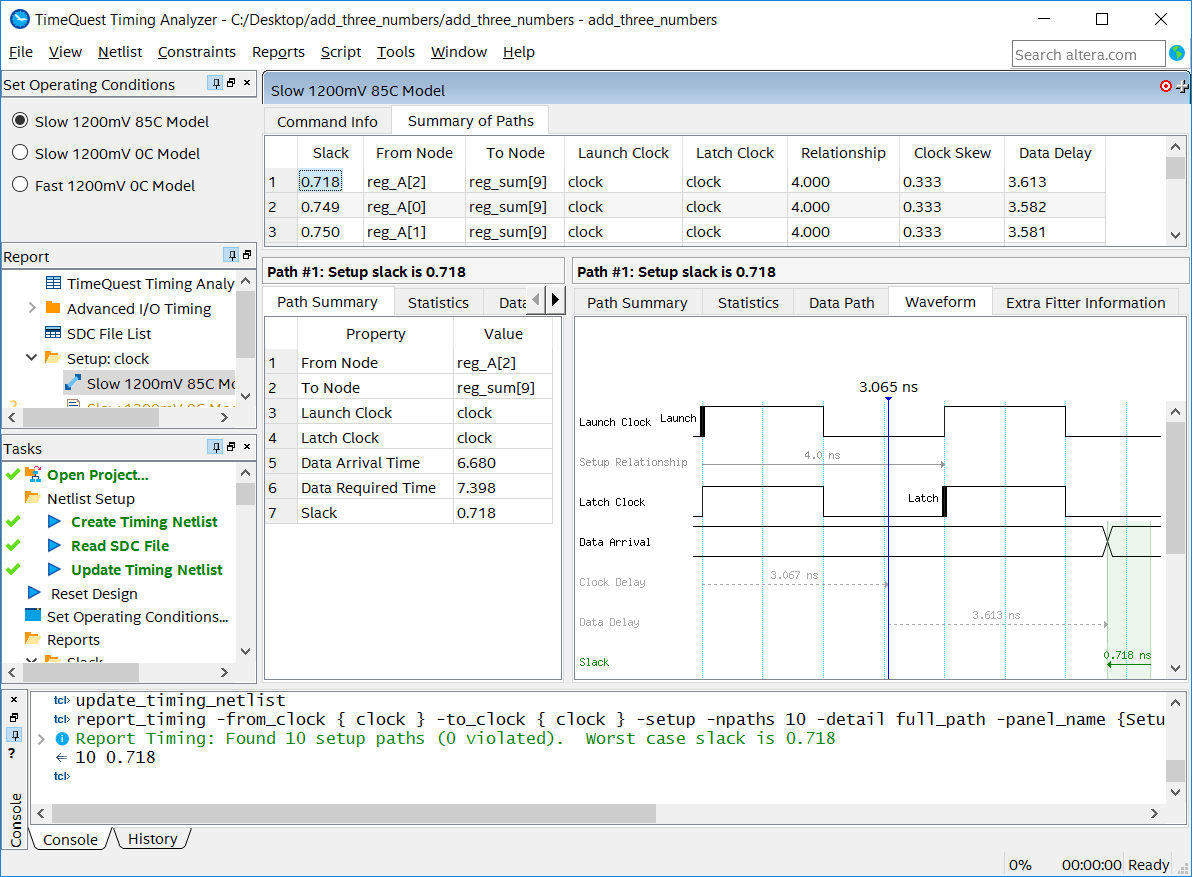
\includegraphics[scale=0.5]{figures/SB9.png}
\end{center}
\caption{Updated compilation results with the 4 ns clock period constraint.}
\label{fig:SB9}
\end{figure}

\newpage
\section{The TimeQuest Graphical User Interface}
\label{sec:TQGUI}

In the above sections we accessed TimeQuest via the Quartus Prime Compilation Report. Another
way to open the TimeQuest GUI is to use the command {\sf Tools > TimeQuest Timing Analyzer}
from the main Quartus Prime window. The TimeQuest window shown in Figure~\ref{fig:5}, will appear.

\begin{figure}[H]
\begin{center}
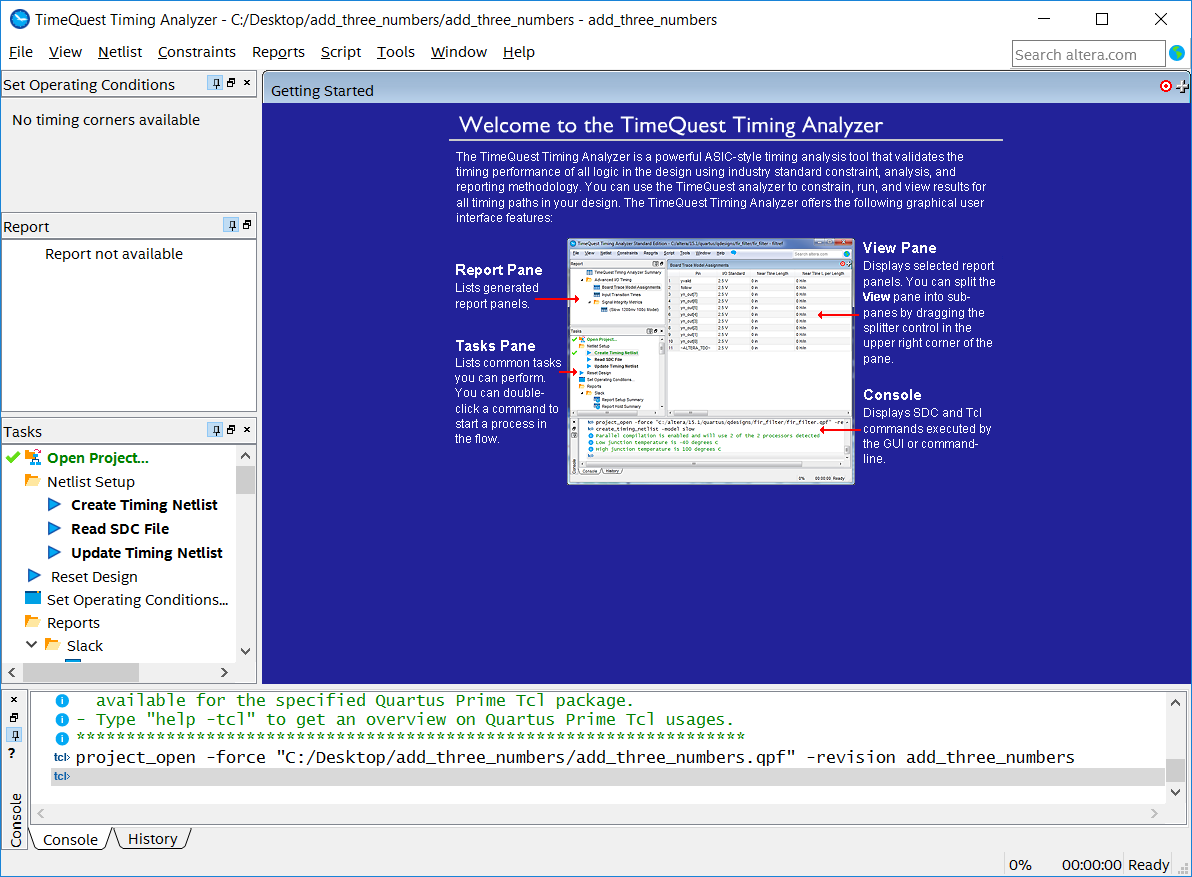
\includegraphics[scale=0.5]{figures/figure5.png}
\end{center}
\caption{TimeQuest window.}
\label{fig:5}
\end{figure}

To demonstrate some of the commands available in the TimeQuest GUI, we go through a set of basic 
steps to obtain timing data for the example design. In the Tasks pane, begin by double-clicking
the {\sf Create Timing Netlist} command to create a timing netlist, which will be used to perform 
the analysis. Note that while this netlist was generated automatically when performing a timing 
analysis as described in the previous sections, the netlist can also be generated manually 
by using the Tasks pane. Next double-click {\sf Read SDC File} to instruct the analyzer to 
read a Synopsys Design Constraints (SDC) file and apply the constraints during analysis.
The SDC file can be edited manually (using any text editor) at any time, and the timing
analysis can then be re-run using the new constraints. 
Finally, double-click the {\sf Update Timing Netlist} command to use the specified 
constraints to determine which parts of the circuit fail 
to meet them. Once the timing netlist is updated, reports can be generated.

\subsection{Timing Analysis Reports}

To generate a report, double-click on a report name in the Tasks pane. 
For example, double-click on the {\sf Report Setup Summary}. This command
will bring up a window in the view pane as shown in Figure~\ref{fig:7}. Right-click on the
{\it clock} name then click on {\sf Report Timing...} to open the Report Timing dialog in Figure~\ref{fig:9}. Although we previously 
showed this dialog in Figure~\ref{fig:SB2} we now describe it in more detail. 

\begin{figure}[H]
\begin{center}
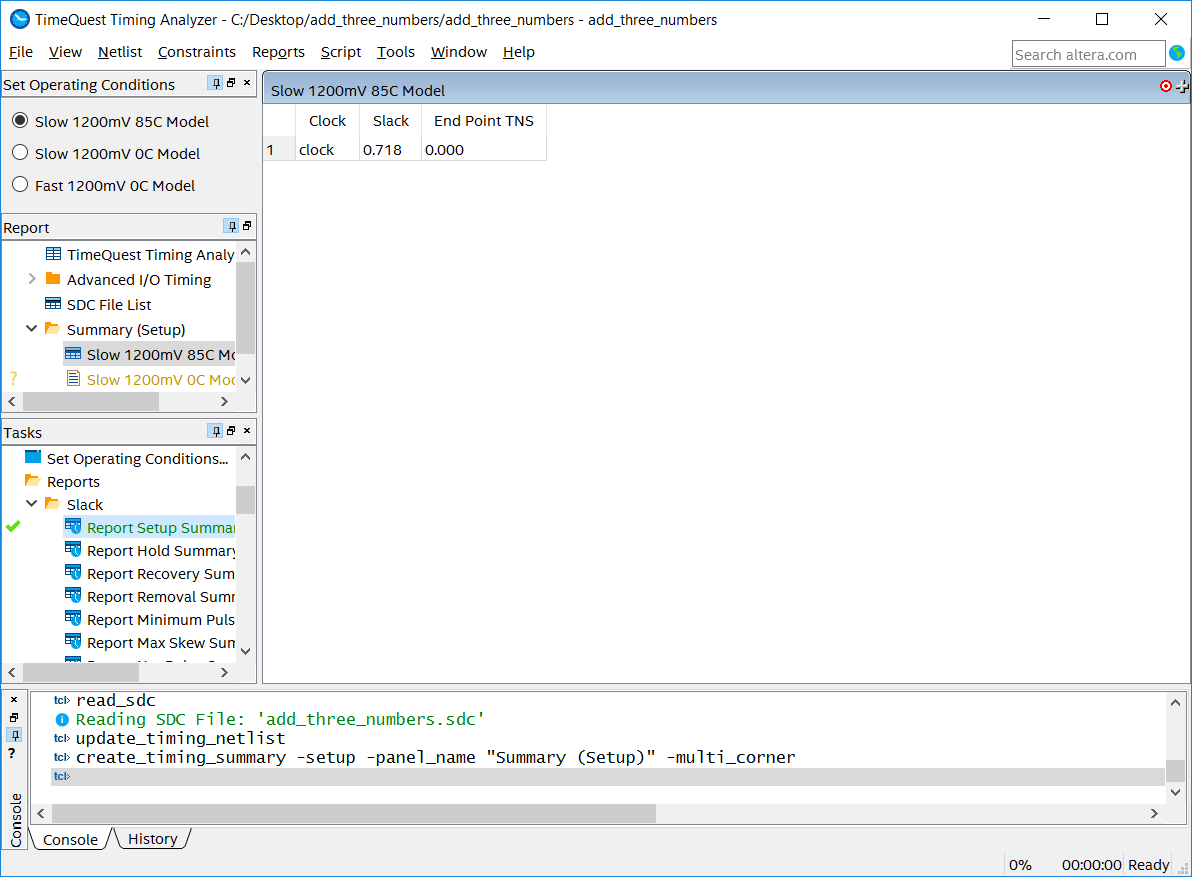
\includegraphics[scale=0.5]{figures/figure7.png}
\end{center}
\caption{Setup summary.}
\label{fig:7}
\end{figure}

There are several fields in Figure~\ref{fig:9} that help specify the data to be reported. The 
first field is the {\sf Clocks} field, which specifies the types of paths that will be reported. 
More precisely, it specifies the clock signal at the source flip-flops ({\sf From clock}) 
and the clock signal at the destination flip-flops ({\sf To clock}).  For this example, choose 
the signal named {\it clock} for the 
{\sf To clock} and {\sf From clock} fields. This will limit the reporting to the 
register-to-register paths only.

\begin{figure}[H]
\begin{center}
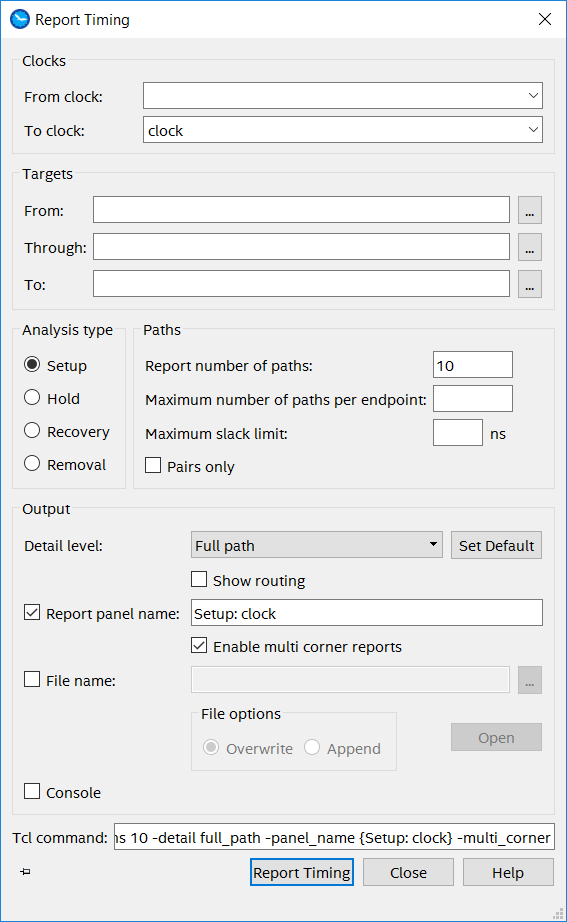
\includegraphics[scale=0.4]{figures/figure9.png}
\end{center}
\caption{Timing report generation window.}
\label{fig:9}
\end{figure}

The next field is the {\sf Targets} field. It can be used to refine the report by focusing 
only on certain paths in the design. We can specify the starting
and the ending point of the paths of interest by filling the {\sf From} and {\sf To} fields. 
In addition, we can look at only the paths that pass through certain
nodes in the design. For this example, we leave these fields blank to indicate that every path 
should be taken into account for the report.

The next two fields are the {\sf Analysis type} and {\sf Paths} fields. The {\sf Analysis type} 
field specifies if the report should contain setup, hold,
recovery, or removal information. Each of these analyses looks for distinct timing 
characteristics in your design. For example, the setup analysis determines if the data arrives 
at a flip-flop sufficiently early for the flip-flop to store it reliably, given a clock period. 
On the other hand, the hold analysis determines if the data input at any given flip-flop remains 
stable after the positive edge of the clock long enough for the data to be
stored in a flip-flop reliably. The {\sf Paths} field specifies the maximum number of paths to 
be reported and the maximum slack required for a path to be included in the report. For this 
example, choose the type of analysis to be {\sf Setup} and select 10 paths to be reported. This 
will generate a setup analysis report and show 10 paths with the least slack.

The next set of fields specify the {\sf Output} format and the level of detail in the report. 
The output could be to a window or a file. Set the Detail level to {\sf Path Only}, then set 
the output to a window by checking the {\sf Report panel name} check box (and not 
the {\sf File name} check box). The window should be named {\sf Setup: clock} by default,
and that name will identify the report in the report pane.

Finally, the last field is the {\sf Tcl command} field. This field shows a command that will 
be executed to generate the requested report. You do not need to edit this field. 

\subsection{Creating Timing Constraints in the TimeQuest GUI}

Timing constraints can be entered by using the {\sf Constraints} menu in the 
TimeQuest GUI.  To assign a clock constraint, select {\sf Create Clock...} from the 
{\sf Constraint} menu. A window shown in Figure~\ref{fig:12} will appear.

\begin{figure}[H]
\begin{center}
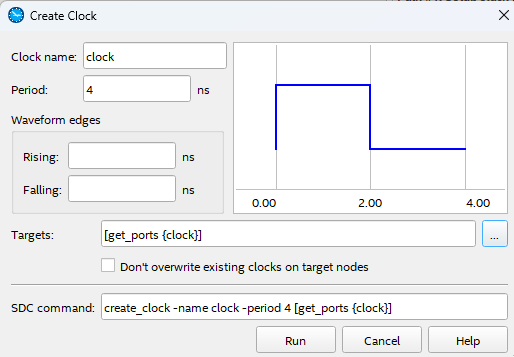
\includegraphics[scale=0.65]{figures/figure12.png}
\end{center}
\caption{TimeQuest window to create a clock constraint.}
\label{fig:12}
\end{figure}

In the figure the clock constraint is given the name {\it clock} in the top field. The
clock period is assigned to be 4 ns in the field below. The next two fields define the time
at which the clock changes from 0 to 1 and 1 to 0. Leaving these fields empty indicates that 
the rising edge of the clock should appear at time 0, and the falling edge at one half of 
the clock period. Finally, the {\sf Targets} field is set to the signal name {\it clock} as 
shown in the figure, to indicate that the given constraint is for the signal named {\it clock}. 
Pressing the {\sf Run} button applies the constraint. The constraint can be saved into an SDC file by double-clicking on the {\sf Write SDC File...} task as 
shown in Figure~\ref{fig:13}.

\begin{figure}[H]
\begin{center}
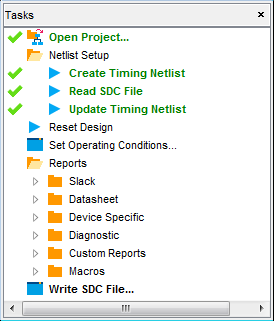
\includegraphics[scale=0.6]{figures/figure13.png}
\end{center}
\caption{Saving a constraints file.}
\label{fig:13}
\end{figure}

Once the constraints file is saved, it can be used by Quartus~Prime when compiling a project. This 
is done in Quartus~Prime by going into {\sf Assignments > Settings... > TimeQuest Timing Analyzer}, 
and adding the SDC file to the TimeQuest timing analyzer settings as shown 
in Figure~\ref{fig:14}. The Quartus Prime project can then be recompiled to use the constraint.

\begin{figure}[H]
\begin{center}
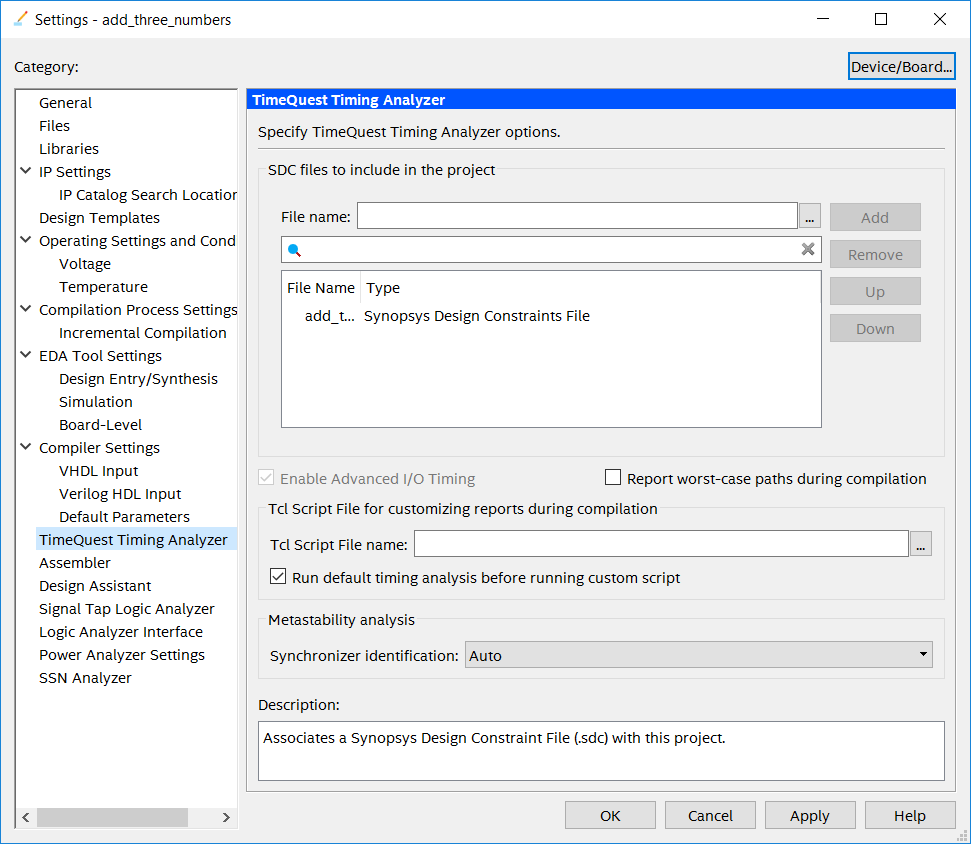
\includegraphics[scale=0.55]{figures/figure14.png}
\end{center}
\caption{Including a constraints file in Quartus Prime project.}
\label{fig:14}
\end{figure}

\section{Circuits with Multiple Clock Signals}
\label{sec:mult}

TimeQuest is capable of analyzing circuits that contain multiple clocks. This includes cases where 
the designer uses several clocks, or where clock signals are generated automatically to 
support features such as the SignalTap II Logic Analyzer or a JTAG* interface. Should the reader 
work with such designs, it is important to note that the experience with TimeQuest may differ 
from that described above. In designs with multiple clocks, it is important to apply constraints
to each clock before performing timing analysis. Doing so will make the analyzer provide 
the same reports as described in previous sections.

\section{Conclusion}

This tutorial demonstrated the basic use of the TimeQuest timing analyzer. While the descriptions 
of timing analysis and setting up timing constraints were limited to clock constraints in a 
simple circuit, TimeQuest provides even more powerful tools to specify timing constraints 
for larger and more complex designs.

% Copyright and Trademark

%\newcommand{\datePublished}{Mar 2022}

\newcommand{\versnum}{21.1} %version number quartus/AMP
\newcommand{\quartusname}{Quartus\textsuperscript{\textregistered} Prime}	
\newcommand{\textBar}{For \quartusname{} \versnum{}}
\newcommand{\thisyear}{2022 } %for copyright
\newcommand{\company}{FPGAcademy.org}
\newcommand{\longteamname}{FPGAcademy.org}
\newcommand{\teamname}{FPGAcademy}
\newcommand{\website}{FPGAcademy.org}

\newcommand{\productAcronym}{AMP}
\newcommand{\productNameShort}{Monitor Program}

\newcommand{\productNameMedTM}{Monitor Program}
\newcommand{\productNameMed}{Monitor Program}

%\newcommand{\headerLogoFilePath}[1]{#1/FPGAcademy.png}



%%%%%%%%%%%%%%%%%%%%%%%%%%%%%%%%%%%%%%%%
%%% FPGAcademy Copyright Information %%%
%%%%%%%%%%%%%%%%%%%%%%%%%%%%%%%%%%%%%%%%

%Always put the copyright on a new page (clear page), with some vertical space from top
\clearpage
\vspace{1in}

\noindent

Copyright {\copyright} FPGAcademy.org. All rights reserved. FPGAcademy and the FPGAcademy logo are trademarks of  FPGAcademy.org.  This document is being provided on an ``as-is'' basis and as an accommodation and therefore all warranties, representations or guarantees of any kind (whether express, implied or statutory) including, without limitation, warranties of merchantability, non-infringement, or fitness for a particular purpose, are specifically disclaimed.

%FPGAcademy assumes no responsibility or liability arising out of the application or use of any information,  product,  or  service  described  herein  except  as  expressly  agreed  to  in  writing  by  FPGAcademy.



**Other names and brands may be claimed as the property of others.




\end{document}
